\documentclass{beamer} 
\usepackage[utf8]{inputenc}
\usepackage[francais]{babel}
\usepackage[T1]{fontenc}
\usepackage{graphicx}

%\useoutertheme{split}
%\usecolortheme{whale}
%\setbeamercolor*{titlelike}{parent=structure}

\setbeamertemplate{footline}[frame number]

\usetheme{Madrid}

\useinnertheme{rectangles}
\setbeamertemplate{itemize subitem}[triangle]
\setbeamertemplate{itemize subsubitem}[circle]

%\usecolortheme[RGB={21, 101, 178}]{structure} 

%\setcounter{tocdepth}{1}

\AtBeginSection[]{
	%\begin{frame}{~}
		%\tableofcontents[current]
		%\begin{center}
			%\huge\insertsection
		%\end{center}
	%\end{frame}
	
	\begin{frame}{Plan}
		\begin{columns}[t]
			\begin{column}{5cm}
				\tableofcontents[sections={1-5},currentsection, hideothersubsections]
			\end{column}
			\begin{column}{5cm}
				\tableofcontents[sections={6-9},currentsection, hideothersubsections]
			\end{column}
		\end{columns}
	\end{frame}
}



\title[Projet tuteuré]{Projet tuteuré}
\subtitle[Projet Tuteuré]{iutbm, introduction ludique à la recherche opérationnelle}
\author[]{VOISIN Julien, BENOIT Marine, NOWINSKI David, ZAMBELLI Cédric, SID Ali, DUROSSIER Florien}
\institute{IUT informatique Belfort}
\date{26 mars 2012}
%\logo{
\includegraphics[width=2cm]{iut_bm.jpg}}

\begin{document}

\begin{frame}{~}
	\titlepage
\end{frame}

%
% Ne pas oublier les remerciements à l'oral !
%

\begin{frame}{Plan}
	\begin{columns}[t]
		\begin{column}{5cm}
			\tableofcontents[sections={1-5}, hideothersubsections]
		\end{column}
		\begin{column}{5cm}
			\tableofcontents[sections={6-9}, hideothersubsections]
		\end{column}
	\end{columns}
\end{frame}

\section{Introduction}
	\begin{frame}{Introduction}
		\begin{itemize}
			\setlength{\itemsep}{0.5cm}
			\item La recherche opérationnelle fait partie de la vie de tout les jours;
			\pause
			\item Mais beaucoup l'ignorent;
			\pause
			\item But du projet : sensibiliser les gens à la recherche
			    opérationnelle.
		\end{itemize}
	\end{frame}

\section{Présentation}
	\subsection{Sujet}
		\begin{frame}{Présentation - Sujet}
			\begin{itemize}
				\setlength{\itemsep}{1cm}
				\item Définir des problèmes pertinents ;
				\item Implémenter les algorithmes ;
				\item Présenter de façon ludique.
			\end{itemize}
		\end{frame}
\section{Cahier des charges}
	\subsection{Objectifs}
		\begin{frame}{Cahier des charges - Objectifs généraux}
			\begin{itemize}\setlength{\itemsep}{0.75cm}
                \item Ludisme
                \item Sensibilisation
                \item Accessibilité
                \item Portabilité
			\end{itemize}
		\end{frame}
	\subsection{Moyens}
		\begin{frame}{Cahier des charges - Moyens}
		    Utiliser des technologies
			\begin{itemize}
				\item libres ;
				\item adaptées ;
				\item gratuites.
			\end{itemize}
		\end{frame}
\section{Analyse}
	\subsection{Solutions existantes}
		\begin{frame}{Analyse - Solutions existantes }
		\begin{center}
		Il n'existe actuellement pas de solutions,
		car le sujet est complexe, et n'est connu que d'une minorité.
		\end{center}
		\end{frame}
	\subsection{Interface}
		\begin{frame}{Analyse - Organisation de l'interface}
			\begin{itemize}
				\setlength{\itemsep}{0.5cm}
				\item Un menu principal ;
				\item Page d'aide ;
				\item Réalisations pas-à-pas;
				\item Proposition de solution.
			\end{itemize}
		\end{frame}
	\subsection{Limites et choix}
		\begin{frame}{Analyse - Limites et choix}
			\begin{itemize}
				\setlength{\itemsep}{0.3cm}
				\item Langage : Python;
					\begin{itemize}
						\item Portabilité ;
						\item Rapidité de développement ;
						\item Langage connu.
					\end{itemize}
				\item Bibliothèque : \emph{pygame} :
					\begin{itemize}
						\item Bibliothèque complète ;
						\item Libre ;
						\item Reconnue;
						\item Simple d'utilisation.
					\end{itemize}
				\item Problèmes :
					\begin{itemize}
						\item Voyageur de commerce
						\item Couplage
						\item Plus court chemin
						\item Ordonnancement
					\end{itemize}
			\end{itemize}
		\end{frame}
\section{Organisation}
	\begin{frame}{Organisation}
		\begin{itemize}
			\setlength{\itemsep}{0.75cm}
			\item Répartition des tâches :
			\begin{itemize}
			\setlength{\itemsep}{0.3cm}
				\item Découpage des tâches ;
				\item Répartition par binômes.
			\end{itemize}
			\item Plate-forme collaborative de travail : \emph{git}
			\begin{itemize}
			\setlength{\itemsep}{0.3cm}
				\item Documentation ;
				\item Développement ;
				\item Tickets.
			\end{itemize}
		\end{itemize}
	\end{frame}

\section{Réalisation}
    \subsection{Interface}
        \begin{frame}{Interface}
            \begin{itemize}
	            \item Menu clair
	            \item Raccourcis clavier
	            \item Aide contextuelle
            \end{itemize}
        \end{frame}
    \subsection{Voyageur de commerce}
    \begin{frame}
        \frametitle{Voyageur de commerce}
        \begin{columns}
            \begin{column}{0cm}
                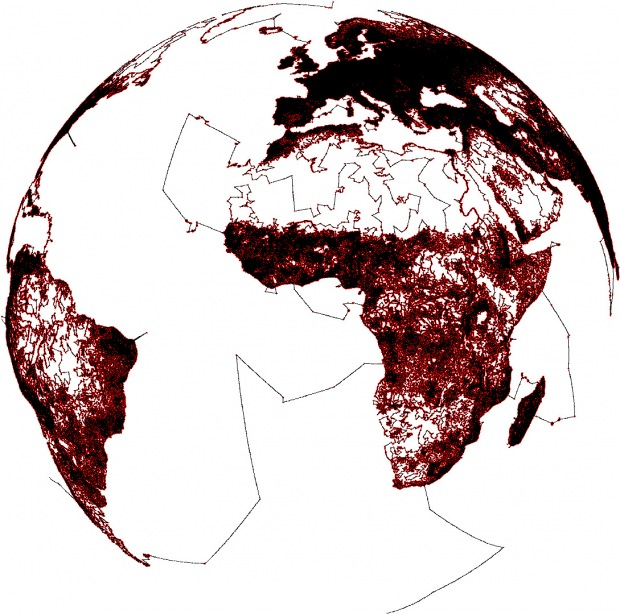
\includegraphics[width=3cm]{images/wts.jpg}
            \end{column}
            \begin{column}{8cm}
                \begin{description}\itemsep15pt
                    \item Problème NP-Complet
                    \item Résolution gloutonne optimisée
                    \item Résolution en arrière plan
                \end{description}
            \end{column}
        \end{columns}
    \end{frame}

	\subsection{Plus court chemin}
		\begin{frame}{Plus court chemin}
        \begin{columns}
            \begin{column}{0cm}
                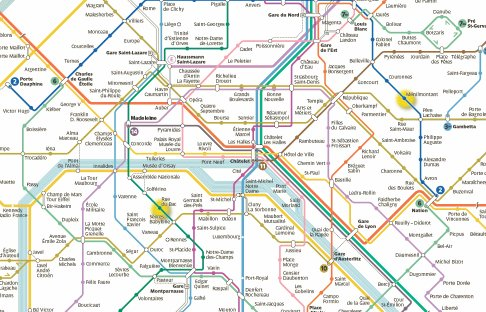
\includegraphics[width=3cm]{images/metro.jpg}
            \end{column}
            \begin{column}{8cm}
                \begin{description}\itemsep15pt
                    \item Problème Polynomial
                    \item Résolution par Dijkstra
                    \item Résolution en arrière plan
                \end{description}
            \end{column}
        \end{columns}
		\end{frame}
	\subsection{Couplage}
		\begin{frame}{Couplage}
           \begin{columns}
            \begin{column}{0cm}
                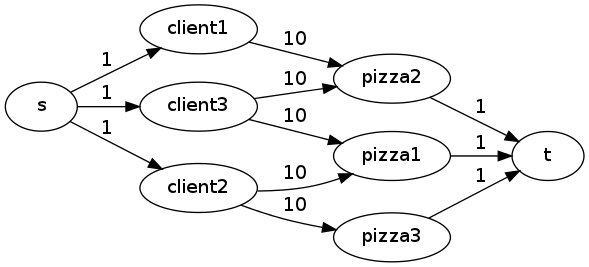
\includegraphics[width=3cm]{images/exemple_couplage.png}
            \end{column}
            \begin{column}{8cm}
                \begin{description}\itemsep15pt
                    \item Problème Polynomial
                    \item Résolution par Ford Fulkerson
                    \item Résolution en arrière plan
                \end{description}
            \end{column}
        \end{columns}
		\end{frame}
	\subsection{Ordonnancement}
		\begin{frame}{Ordonnancement}
        \begin{columns}
            \begin{column}{0cm}
                
\includegraphics[width=3cm]{images/knapsack.png}
            \end{column}
            \begin{column}{8cm}
                \begin{description}\itemsep15pt
                    \item Problème Pseudo-Polynomial
                    \item Résolution par programmation dynamique
                    \item Résolution en arrière plan
                \end{description}
            \end{column}
        \end{columns}
		\end{frame}

\section{Problèmes rencontrés}
\subsection{Git(hub)}
	\begin{frame}{Git(hub)}
	    Utiliser une forge logicielle n'est pas chose aisée :
		\begin{itemize}
		\setlength{\itemsep}{0.5cm}
			\item Branches ;
			\item Travail en parallèle ;
			\item Tickets.
		\end{itemize}
	\end{frame}
\subsection{Problèmes humains}
	\begin{frame}{Humain}
	    \begin{itemize}
		\setlength{\itemsep}{1cm}
	        \item Répartition de la charge de travail
	        \item Motivations inégales
	        \item Soucis de communication
        \end{itemize}
	\end{frame}


\section{Bilans}
\subsection{Bilan technique}
	\begin{frame}{Bilan technique}
		\begin{itemize}
		\setlength{\itemsep}{0.3cm}
			\item Le Python nous a permis de développer rapidement et efficacement;
			\item Les questions de portabilité ne se sont pas posées ;
			\item Le code est propre et documenté.
		\end{itemize}
	\end{frame}
\subsection{Bilan humain}
	\begin{frame}{Bilan humain}
		\begin{itemize}
			\item Travail d'équipe parcellaire ;
			\item Réunions/échanges
			\vspace{1cm}
			\item Travail en autonomie/binôme
		\end{itemize}
	\end{frame}
\subsection{Bilan pédagogique}
	\begin{frame}{Bilan pédagogique}
		\begin{itemize}
		\setlength{\itemsep}{0.3cm}
			\item Approfondissement des bases en \emph{Python} ;
			\item Prise en main d'une bibliothèque totalement inconnue :
			\emph{pygame} ;
			\vspace{1cm}
			\item Utilisation d'un gestionnaire de version ;
			\item Documentation du code
			\item Travail en équipe
            \item Apprentissages d'algorithmes complexes ;
		\end{itemize}
	\end{frame}
\subsection{Perspectives d'évolution}
	\begin{frame}{Perspectives d'évolution}
		Quelques idées que nous n'avons pas eu le temps d'implémenter :
		\begin{itemize}
		\setlength{\itemsep}{0.3cm}
			\item Implémenter plus d'algorithmes ;
			\item Internationalisation ;
			\item Meilleure interface;
            \item Selecteur de niveau.
		\end{itemize}
	\end{frame}

\section{Conclusion}
	\begin{frame}{Conclusion}
		\begin{itemize}
		\setlength{\itemsep}{0.4cm}
			\item Approfondissement de nos bases en Python ;
			\item Découverte en autonomie de la bibliothèque \emph{pygame} ;
			\item Découverte de méthodes/techniques de développement en groupe ;
			\item Résultats bien meilleurs que nos espérances !
		\end{itemize}
	\end{frame}

\end{document}
